\section{upLaTeX実例章}

\subsection{概要}

この章では、upLaTeXにおける画像参照と参考文献管理のベストプラクティスを実装しています。

\subsection{画像参照の実装}

図\ref{fig:test_image_up}に示すテスト画像は、\texttt{graphicspath}による相対パス参照で読み込まれています。

\begin{figure}[htbp]
    \centering
    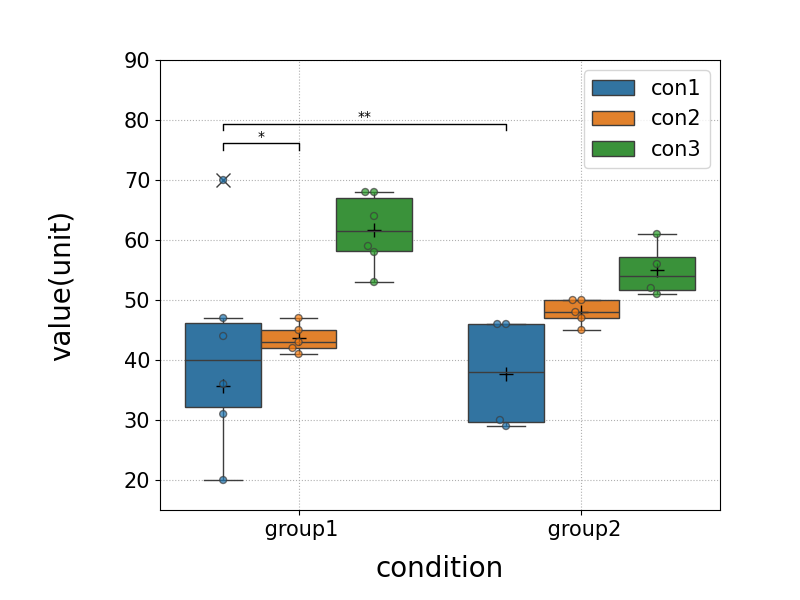
\includegraphics[width=0.7\textwidth,bb=0 0 512 384]{test/test.png}
    \caption{upLaTeX用テスト画像}
    \label{fig:test_image_up}
\end{figure}

upLaTeXでは日本語文字との組み合わせにおいても、適切な画像配置が可能です。

\subsection{文献参照}

参考文献の例として、Doe~\cite{example}による研究を引用します。upLaTeXでは\texttt{pbibtex}により日本語を含む参考文献も適切に処理されます。

\subsection{技術的特徴}

本文書構造では以下の技術的特徴を実装しています:

\begin{itemize}
    \item \texttt{graphicspath}による画像パス自動解決
    \item 相対パス参照による可搬性の確保
    \item \texttt{pbibtex}による日本語対応文献管理
\end{itemize}

\subsection{まとめ}

upLaTeXを使用することで、従来のpLaTeXの利点を保ちながら、UTF-8エンコーディングによる現代的な日本語文書作成が可能になります。
